\section{Method}

An image $f(u,v)$ can be represented using an illumination-reflectance model. 
\begin{figure}[h!]
\begin{equation}
  f(u,v) = i(u,v) r(u,v)
  \label{eqn:im1}
\end{equation}
\caption{Image $f$ represented with an illumination component $i$ and reflection component $r$}
\end{figure}
The illumination $i(u,v)$ can be characterized as slow changes in the frequency domain or as glooming light in the spatial domain. While the reflection $r(u,v)$ tends to be rapid changes in the frequency domain or as edges in the spatial domain. The homomorphic filter works in the frequency domain and aims to filter out major influences of the illumination $i(u,v)$. This results in a higher contrast and normalized brightness. \\

\subsection{Pre-pocessing of the original image}
To apply the filter the image $f(u,v)$ needs to be transformed into frequency domain. Since the illumination-reflectance model is multiplicative and will result in a convolution in frequency space the image will need to be pre-processed before the transformation.

\begin{figure}[h!]
\begin{equation}
  \mathfrak{F}[f(u,v)] = \mathfrak{F}[i(u,v)] \ast \mathfrak{F}[r(u,v)] 
  \label{eqn:transWithoutLogRes}
\end{equation}
\begin{equation}
  \mathfrak{F}[f(u,v)] \neq \mathfrak{F}[i(u,v)] \mathfrak{F}[r(u,v)] 
  \label{eqn:transWithoutLogErr}
\end{equation}
\caption{Multiplication will become convolution (\ref{eqn:transWithoutLogRes}) in frequency domain and not remain multiplicative.(\ref{eqn:transWithoutLogErr})}
\end{figure}

Applying the logarithmic transformation on the original image results in a transformation of the illumination-reflectance model from multiplicative to additive, Eq \ref{eqn:loga}. The Fourier transform is applied to the resulting image of the logarithmic transform and the illumination-reflectance model is intact and in frequency domain as seen in EQ \ref{eqn:logtrans}
\begin{figure}[h!]
\begin{equation}
  f(u,v) = i(u,v) r(u,v) \xrightarrow{\ln} \ln{f(u,v)} = \ln{i(u,v)} + \ln{r(u,v)} 
  \label{eqn:loga}
\end{equation}
  \begin{equation}
    \begin{split}
      Z(u,v) &= \mathfrak{F} [\ln{f(u,v)}]\\ &= \mathfrak{F}[\ln{i(u,v)}] + \mathfrak{F}[\ln{r(u,v)}]\\ &= F_i(u,v) + F_r(u,v)
    \end{split}
    \label{eqn:logtrans}
  \end{equation}
\caption{image $f$ represented with an illumination component $i$ and reflection component $r$, in Eq \ref{eqn:loga} multiplication becomes additive after logarithmic transform. Eq \ref{eqn:logtrans} shows the result of a fourier and logarithmic transformed image $Z$ and the corresponding illumination and reflection component.}
\end{figure}

Since the images are discrete and the Fourier Transform is applied to infinity, matlab will loop the input image periodically. To avoid aliasing and introduction of errors when applying the filter to the image, the input image is zero padded. Zero Padding the source image using matlabs \verb~padarray~ -function. The amount of zeros padded with the image is calculated using equations \ref{eqn:Ppadded} and \ref{eqn:Qpadded} given in the coursebook\cite[p. 274]{dipBook}. Exempel of zero padding is shown in Figure \ref{fig:zeropadded}.
\begin{figure}[h!]
\begin{equation}
  P \geq 2M -1
  \label{eqn:Ppadded}
\end{equation}
\caption{4.6-31, P: Resulting vertical size of the image, M: vertical size of source image}
\end{figure}

\begin{figure}[h!]
  \begin{equation}
    Q \geq 2N -1
    \label{eqn:Qpadded}
  \end{equation}
  \caption{4.6-31, Q: Resulting horisontal size of the image, N: horizontal size of source image}
\end{figure}

\begin{figure}[h!]
  \begin{center}
    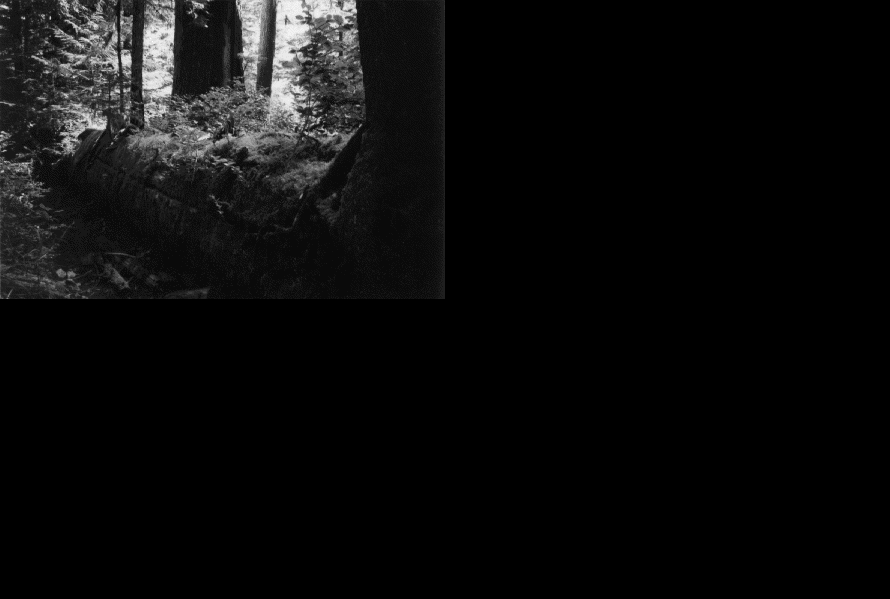
\includegraphics[width=0.6\textwidth]{pics/zeroPadded.png}
  \end{center}
  \cprotect\caption{Original image padded with P-M and Q-N zeros after original matrix using \verb~padarray~ in matlab.}
  \label{fig:zeropadded}    
\end{figure}

The filter used in this project is center positioned. Since matlabs \verb~fft2~ returns the transformed image with the origio in upper left corner, the result must be shifted to apply the filter correctly. Shifting the transformation is done using matlabs \verb~fftshift~

\subsection{The construction of the homomorphic filter}
The filter used to enhanced the image in this project is a highpass gaussian filter,Eq \ref{eqn:gaussian_filter}, with three parameters. 
    \begin{equation}
    \label{eqn:gaussian_filter}
      H(u,v) = \left( \gamma_H - \gamma_L \right) \left[ 1 - e^{- D(u,v) /2 \cdot D_0^2}\right] + \gamma_L 
    \end{equation}

\begin{itemize}
  \item $\gamma_H$ sets the maximum enhancement of high frequencies.
  \item $\gamma_L$ sets the maximum inhibition of low frequencies.
  \item $D_0$ is the cut-of frequency, to control the steepness and width of the gaussian function.
  \item The function $D(u,v)$ calculates the distance from the center of the filter to each element ,$u,v$, in the filter.  
\end{itemize}

\begin{figure}[h!]
  \begin{lstlisting}
    [u, v] = meshgrid(1:q,1:p);
    centerU = ceil(q/2);
    centerV = ceil(p/2);
    gaussianNumerator = ((u - centerU).^2 + (v - centerV).^2);
  \end{lstlisting}
  \label{code:raduv}
  \caption{Matlab code of the distance function $D(u,v)$ used in the filter. p and q is the size of the image after zero padding.}
\end{figure}

\subsection{Applying the filter and the post-processing}

The filter is applied by multiplication in the Frequency domain as seen in Figure \ref{fig:filteringOfImage}. 
\begin{figure}[h!]
  \begin{equation}
    S(u,v) = Z(u,v)H(u,v)
    \label{eqn:applyfilt}
  \end{equation}
  \caption{S: the filtered image, Z: pre-processed image from Eq \ref{eqn:logtrans}, H: highpass guassian filter described in Eq \ref{eqn:gaussian_filter} }
  \label{fig:filteringOfImage}    
\end{figure}

Post-processing consists of four steps.

\begin{enumerate}
  \item Shifting the filtered image to get the origin in top/left corner.
  \item Apply the inverse fourier transform. Crop the zero padding to obtain the original image dimensions.
  \item Crop the zero padding to obtain the original image dimensions.
  \item Inverse logarithmic transformation by taking the exponential function of the result of cropped image.
\end{enumerate}

The result of the post-process is homomorphic filtered image. 